\chapter{General Discussion}\thumbforchapter
\newpage

\section{The (molecular) phylotypic stage}

All models are wrong, but some are useful. 

\begin{figure}[H]
    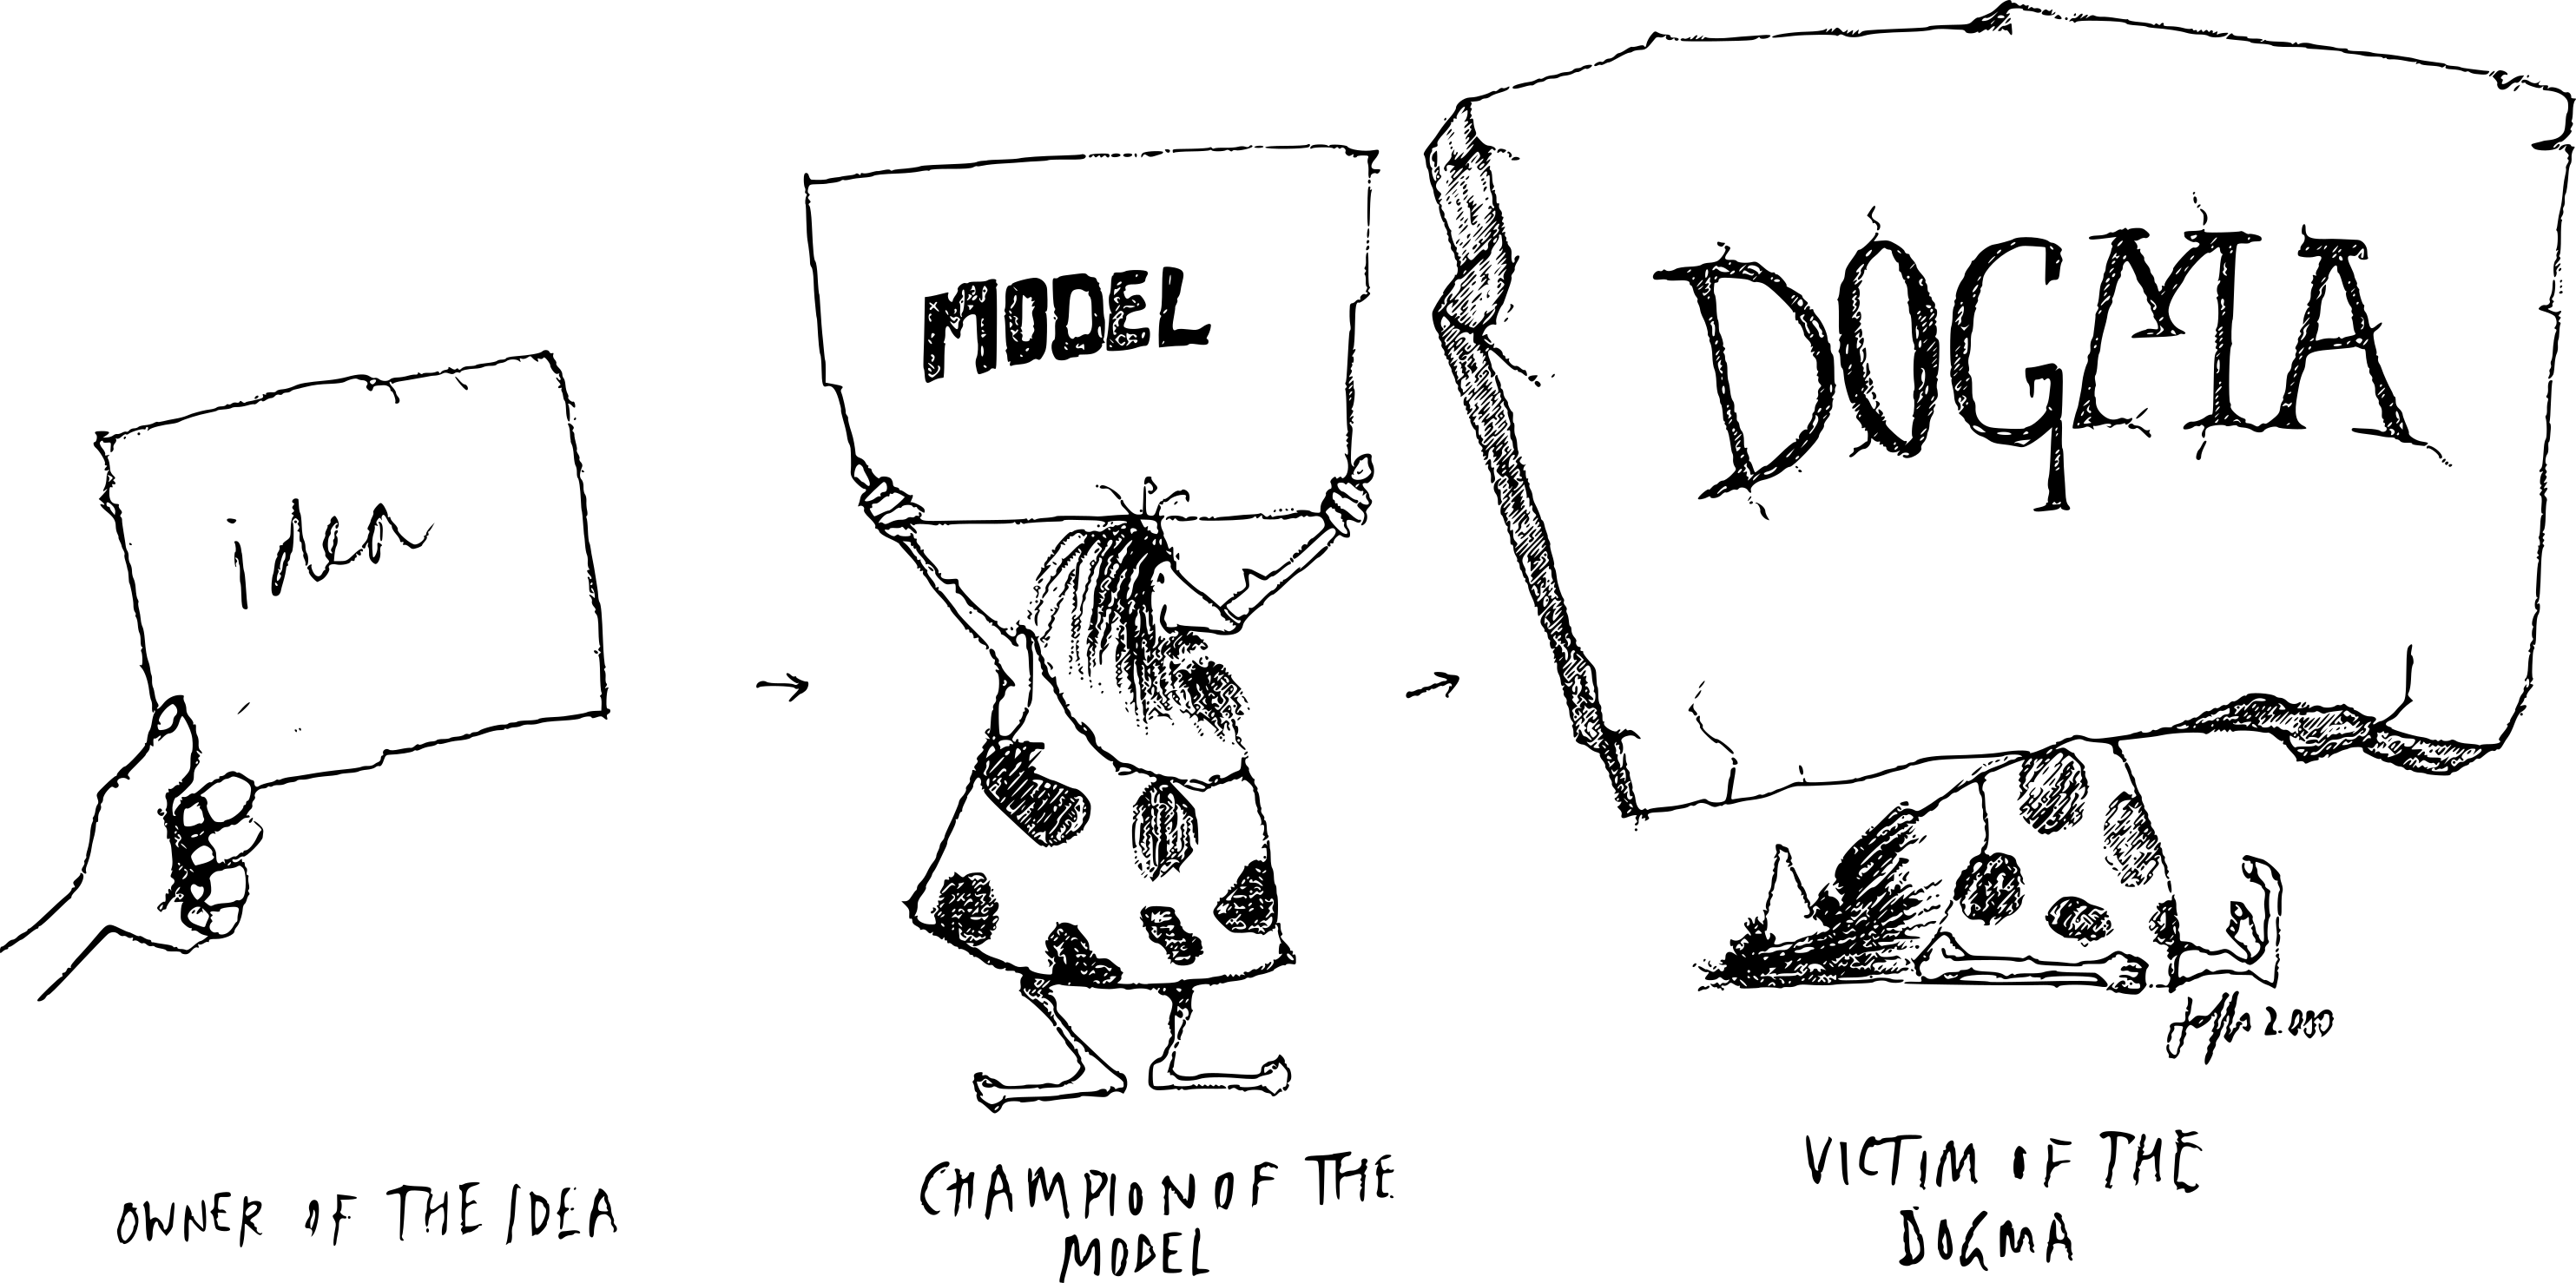
\includegraphics[width=\linewidth]{ch.discussion/imgs/dogma.png}
    \caption{\textbf{The hourglass model as a dogma}. \cite{Caveman2000}}
    \label{fig:dogma}
\end{figure}

\section{scepia: gene regulatory networks}

Almost all gene regulatory approaches are context specific. But in the end a single set of instructions (DNA) for all contexts.

\section{The future of biology}

\subsection{Computational}

\subsection{lack of unified data encode like stuff}

For seq2science paper we tried paper X, Y, Z. DIFFICULT to get similar results.     

% No similarity between replicates:
% https://www.nature.com/articles/s41467-019-12687-4
% 
%  - drosophila sample missing and two other samples swapped
%  - inverse hourglass time orientation has negative values

\subsection{Open Science}

\subsection{Too much descriptive, not enough understanding}

\subsection{Move away from mRNA}

mRNA and protein relation

https://www.biorxiv.org/content/10.1101/2023.05.23.541948v1

cool work of michael levine on xenobots

% https://twitter.com/nimwegenlab/status/1671923176626847744?s=12&t=oyB_faiBr8aHqHcjXZE50A

\begin{figure}[H]
    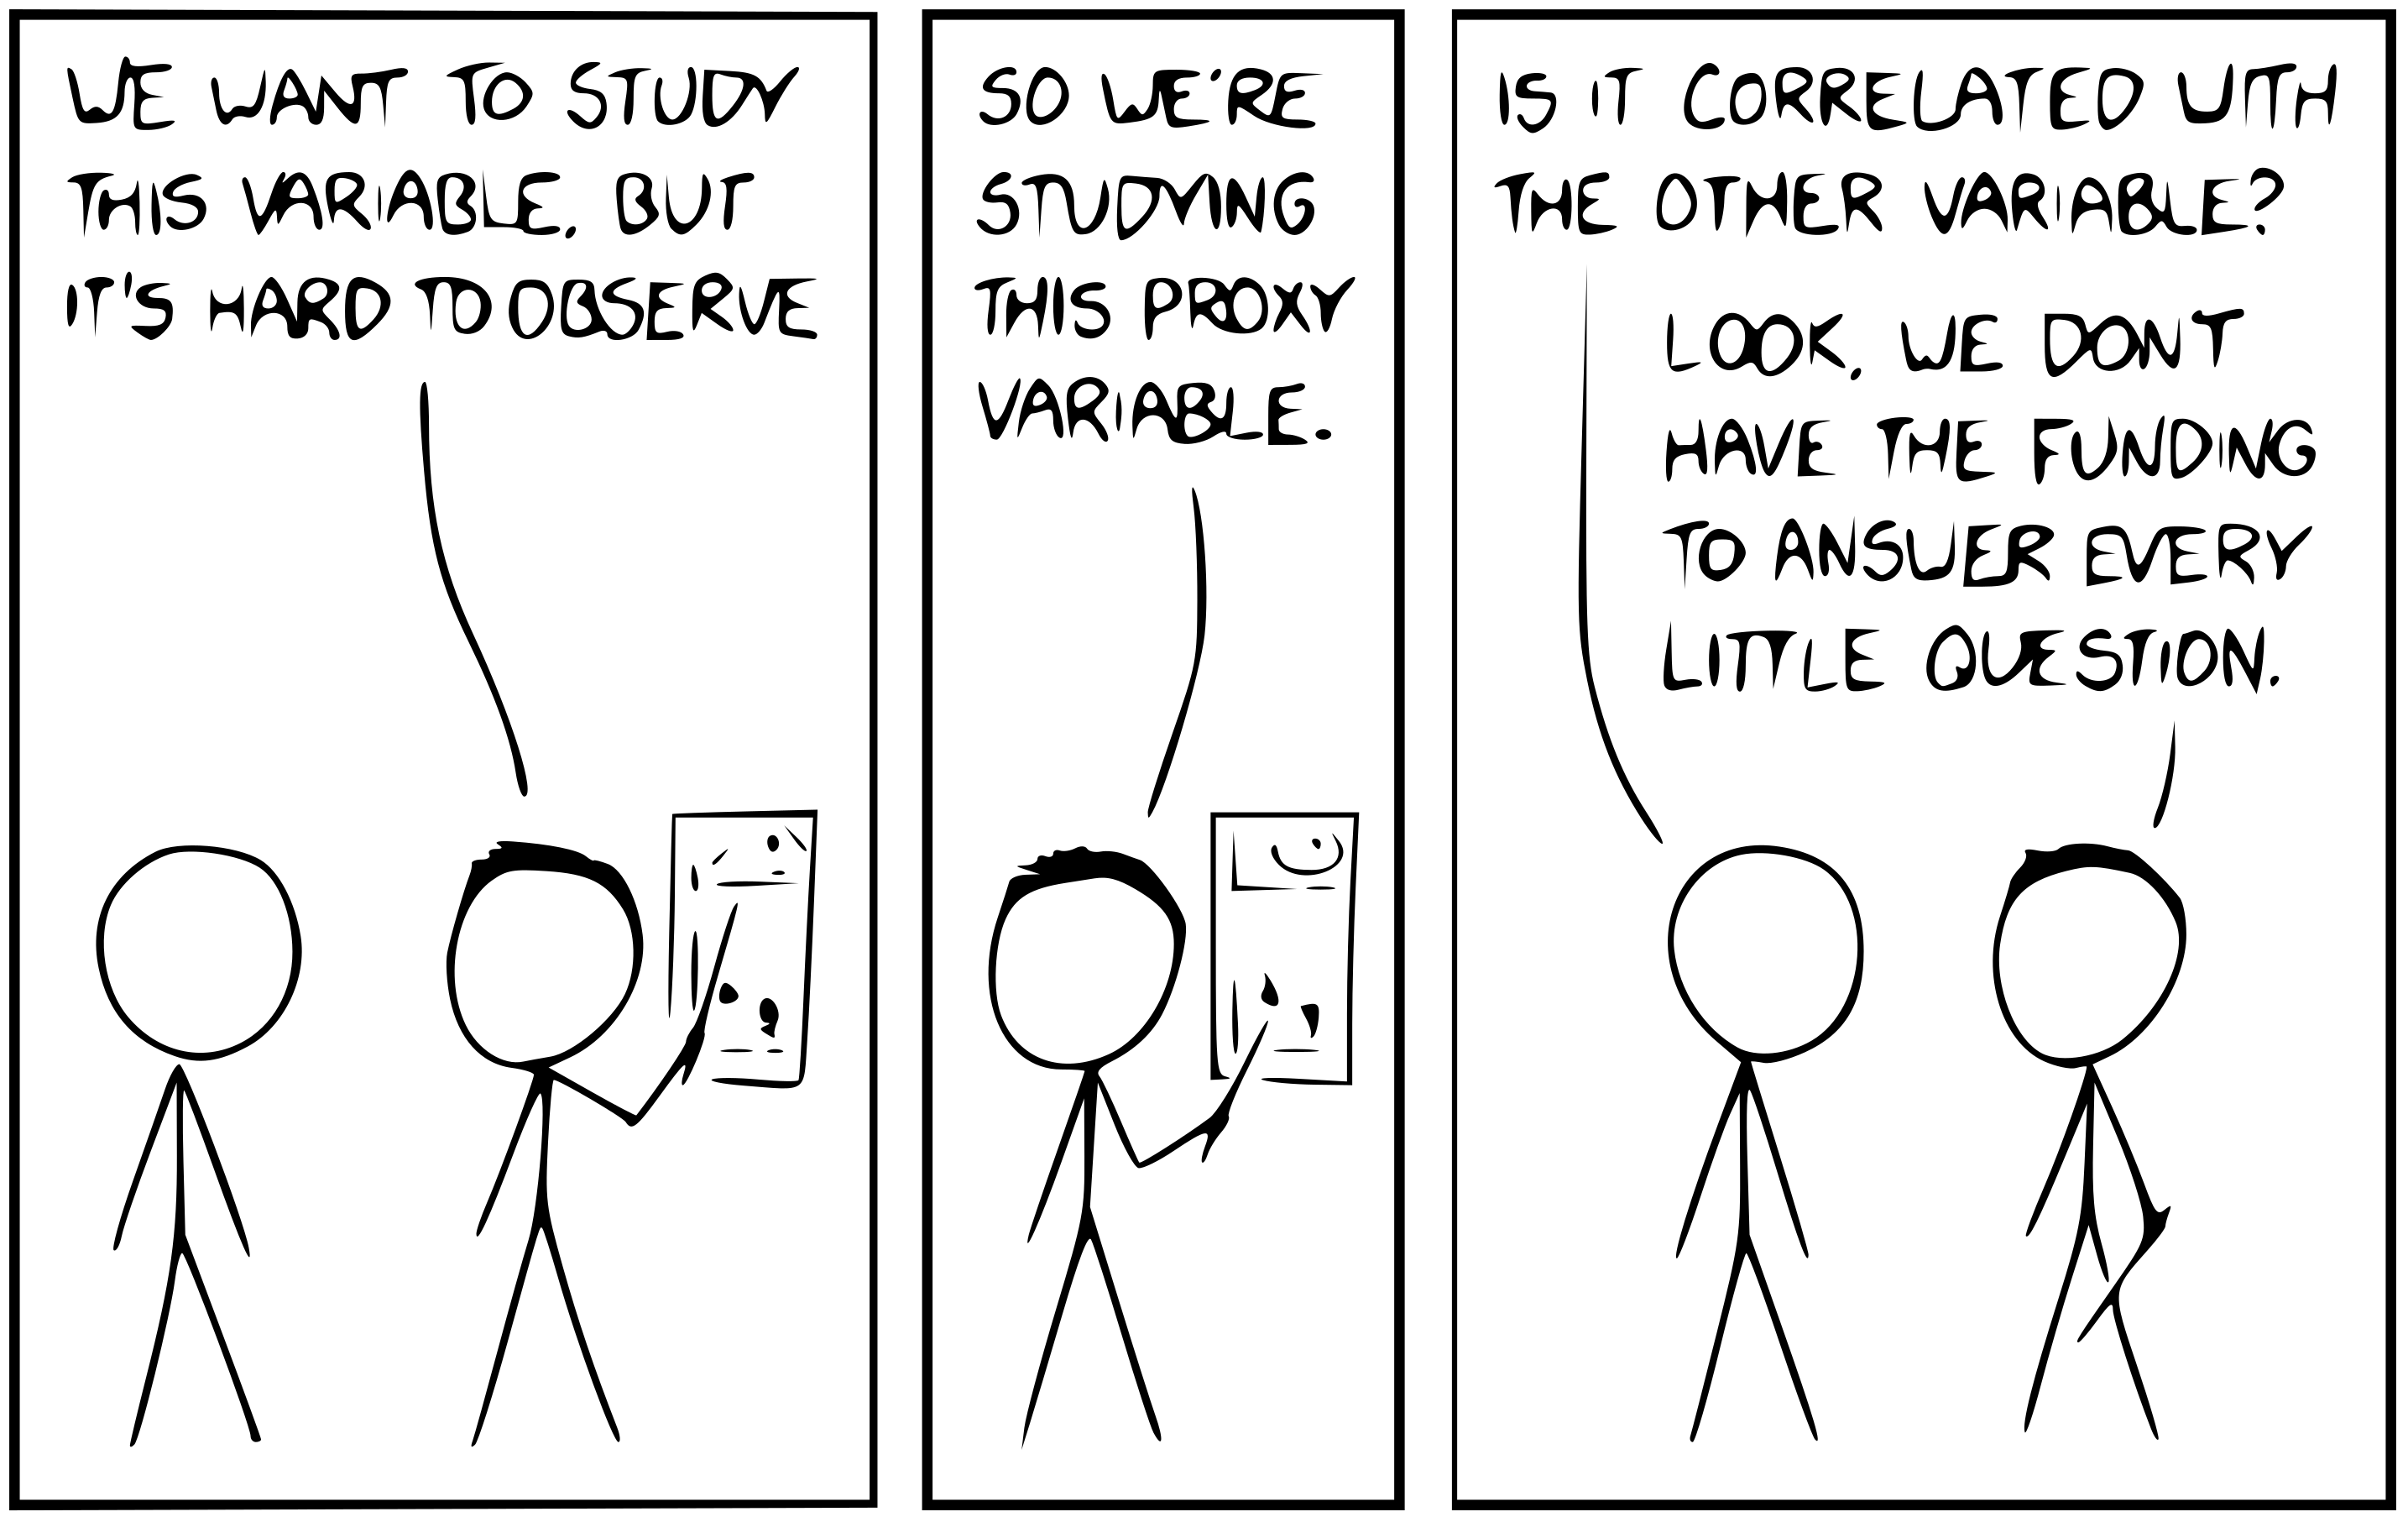
\includegraphics[width=\linewidth]{ch.discussion/imgs/xkcd.png}
    \caption{\textbf{xkcd}. URL: https://xkcd.com/2652}
    \label{fig:xkcd}
\end{figure}

\subsection{Stop blaming "the incentives"}

incentives: https://www.talyarkoni.org/blog/2018/10/02/no-its-not-the-incentives-its-you/

\subsection{Self-correcting}

e.g. wild growth covid papers

papers keep on being cited after retraction or criticism. Number one paper of percentage of genome is functional gives highly criticized ENCODE paper.

highlight cancer genome paper.



% Biology is messy, but that does not mean computational biology has to be.
